%%%%%%%%%%%%%%%%%%%%%%%%%%%%%%%%%%%%%%%%%
% a0poster Landscape Poster
% LaTeX Template
% Version 1.0 (22/06/13)
%
% The a0poster class was created by:
% Gerlinde Kettl and Matthias Weiser (tex@kettl.de)
% 
% This template has been downloaded from:
% http://www.LaTeXTemplates.com
%
% License:
% CC BY-NC-SA 3.0 (http://creativecommons.org/licenses/by-nc-sa/3.0/)
%
%%%%%%%%%%%%%%%%%%%%%%%%%%%%%%%%%%%%%%%%%

%----------------------------------------------------------------------------------------
%	PACKAGES AND OTHER DOCUMENT CONFIGURATIONS
%----------------------------------------------------------------------------------------

\documentclass[a0,landscape]{a0poster}

\usepackage{multicol} % This is so we can have multiple columns of text side-by-side
\columnsep=90pt % This is the amount of white space between the columns in the poster
\columnseprule=3pt % This is the thickness of the black line between the columns in the poster

\usepackage{vwcol}  
\usepackage[svgnames]{xcolor} % Specify colors by their 'svgnames', for a full list of all colors available see here: http://www.latextemplates.com/svgnames-colors

\usepackage{times} % Use the times font
%\usepackage{palatino} % Uncomment to use the Palatino font

\usepackage{graphicx} % Required for including images
\graphicspath{{figures/}} % Location of the graphics files
\usepackage{booktabs} % Top and bottom rules for table
\usepackage[font=small,labelfont=bf]{caption} % Required for specifying captions to tables and figures
\usepackage{amsfonts, amsmath, amsthm, amssymb} % For math fonts, symbols and environments
\usepackage{wrapfig} % Allows wrapping text around tables and figures
\usepackage[compact]{titlesec}
\titlespacing{\section}{0in}{*2}{*0}
\setlength{\parindent}{.5in}
\pagenumbering{gobble}
\linespread{0.65}
\begin{document}

%----------------------------------------------------------------------------------------
%	POSTER HEADER 
%----------------------------------------------------------------------------------------

% The header is divided into three boxes:
% The first is 55% wide and houses the title, subtitle, names and university/organization
% The second is 25% wide and houses contact information
% The third is 19% wide and houses a logo for your university/organization or a photo of you
% The widths of these boxes can be easily edited to accommodate your content as you see fit

\begin{minipage}[b]{0.70\linewidth}
\veryHuge \color{NavyBlue} \textbf{Augmented and Autonomous Vehicle Security} \color{Black}\\ % Title
\huge \textbf{Kevin Gilbert, Christopher Haster, Gilberto Rodriguez III, Hao Chen, Young Chou, Joshua Bryant}\\ % Author(s)
\huge University of Texas at Austin\\ 
\end{minipage}
%
%\begin{minipage}[b]{0.25\linewidth}
%\color{DarkSlateGray}\Large \textbf{Contact Information:}\\
%Department Name\\ % Address
%University Name\\
%123 Broadway, State, Country\\\\
%Phone: +1 (000) 111 1111\\ % Phone number
%Email: \texttt{john@LaTeXTemplates.com}\\ % Email address
%\end{minipage}
%%
\hfill\begin{minipage}[t]{0.10\linewidth}
\begin{flushright}

\includegraphics[width=8cm]{ti_logo} % Logo or a photo of you, adjust its dimensions here
\end{flushright}

\end{minipage}

\vspace{1cm} % A bit of extra whitespace between the header and poster content

%----------------------------------------------------------------------------------------

\begin{multicols}{3} % This is how many columns your poster will be broken into, a poster with many figures may benefit from less columns whereas a text-heavy poster benefits from more

%----------------------------------------------------------------------------------------
%	ABSTRACT
%----------------------------------------------------------------------------------------

\color{Navy} % Navy color for the abstract
-
\section*{Abstract}
\large{
Our research project is focused on highlighting security concerns in augmented and autonomous vehicles. We have developed and built a robotics testbed and simulator on which we can measure and apply real-world data. We primarily focus on the two coupled weak points in augmented automotive cybersecurity: wireless transceiver entry points into an unsecured Controller Area Network (CAN).}

\hfill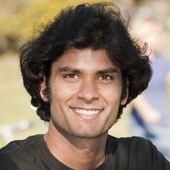
\includegraphics[scale=0.001]{mohit}

%\end{abstract}

%----------------------------------------------------------------------------------------
%	OBJECTIVES
%----------------------------------------------------------------------------------------

\color{DarkSlateGray} % DarkSlateGray color for the rest of the content
%\vspace {-5em}
\section*{Main Objectives}
Our main objectives were to design and implement a testbed on which we could launch security exploits and defenses while providing a retrospective of current automotive cybersecurity. We wished to highlight the inherit dangers of an unsecured CAN bus and demonstrate the necessity of high speed, short-term encryption. Our goals were to create a secured CAN-like protocol within a FPGA coupled with hardware encryption on which we could pipe wireless packets through. We would test this device with a set of wireless transceivers at high speeds in moving vehicles and within our robotics testbed. The realworld data we generated could then be used within a simulator in which we could measure safety and implement a variety of network protocols.

%----------------------------------------------------------------------------------------
%	MATERIALS AND METHODS
%----------------------------------------------------------------------------------------
%\vspace {-3em}
\section*{Modules}

Our primary modules were broken down into: 

\begin{multicols}{2}
\begin{itemize}
\item FPGA -
\subitem CAN Bus
\subitem UART - CAN Packet Translation
\subitem PWM Generation
\subitem Hardware Encryption
\item Wireless Transceivers -
\subitem Data Transmission
\subitem Software Encryption
\item Robotics Testbed -
\subitem Data Measurement
\item Embedded -
\subitem IMU Measurement
\subitem Motor Control (PID)
\subitem Laptop to CAN Bus Interface
\subitem Sensor Interface
\item Simulator -
\subitem Network Timing Constraints
\end{itemize}
\end{multicols}
%------------------------------------------------
	
\section*{Measurements and Data}

We will focus on modular specific system testing and timing constraints collected in this section. The following section will collect this data into a summary of our results.

\begin{vwcol}[widths={0.4,0.6}]
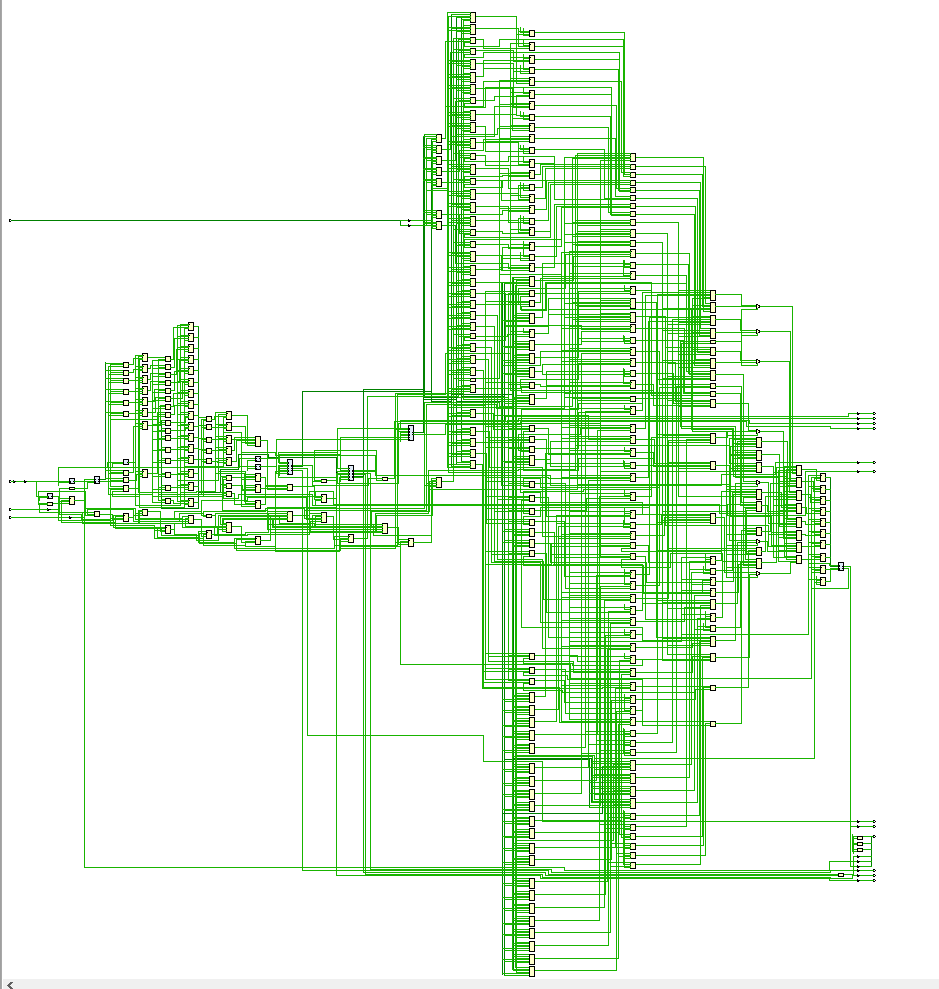
\includegraphics[scale=0.5]{fpga_synth1}
%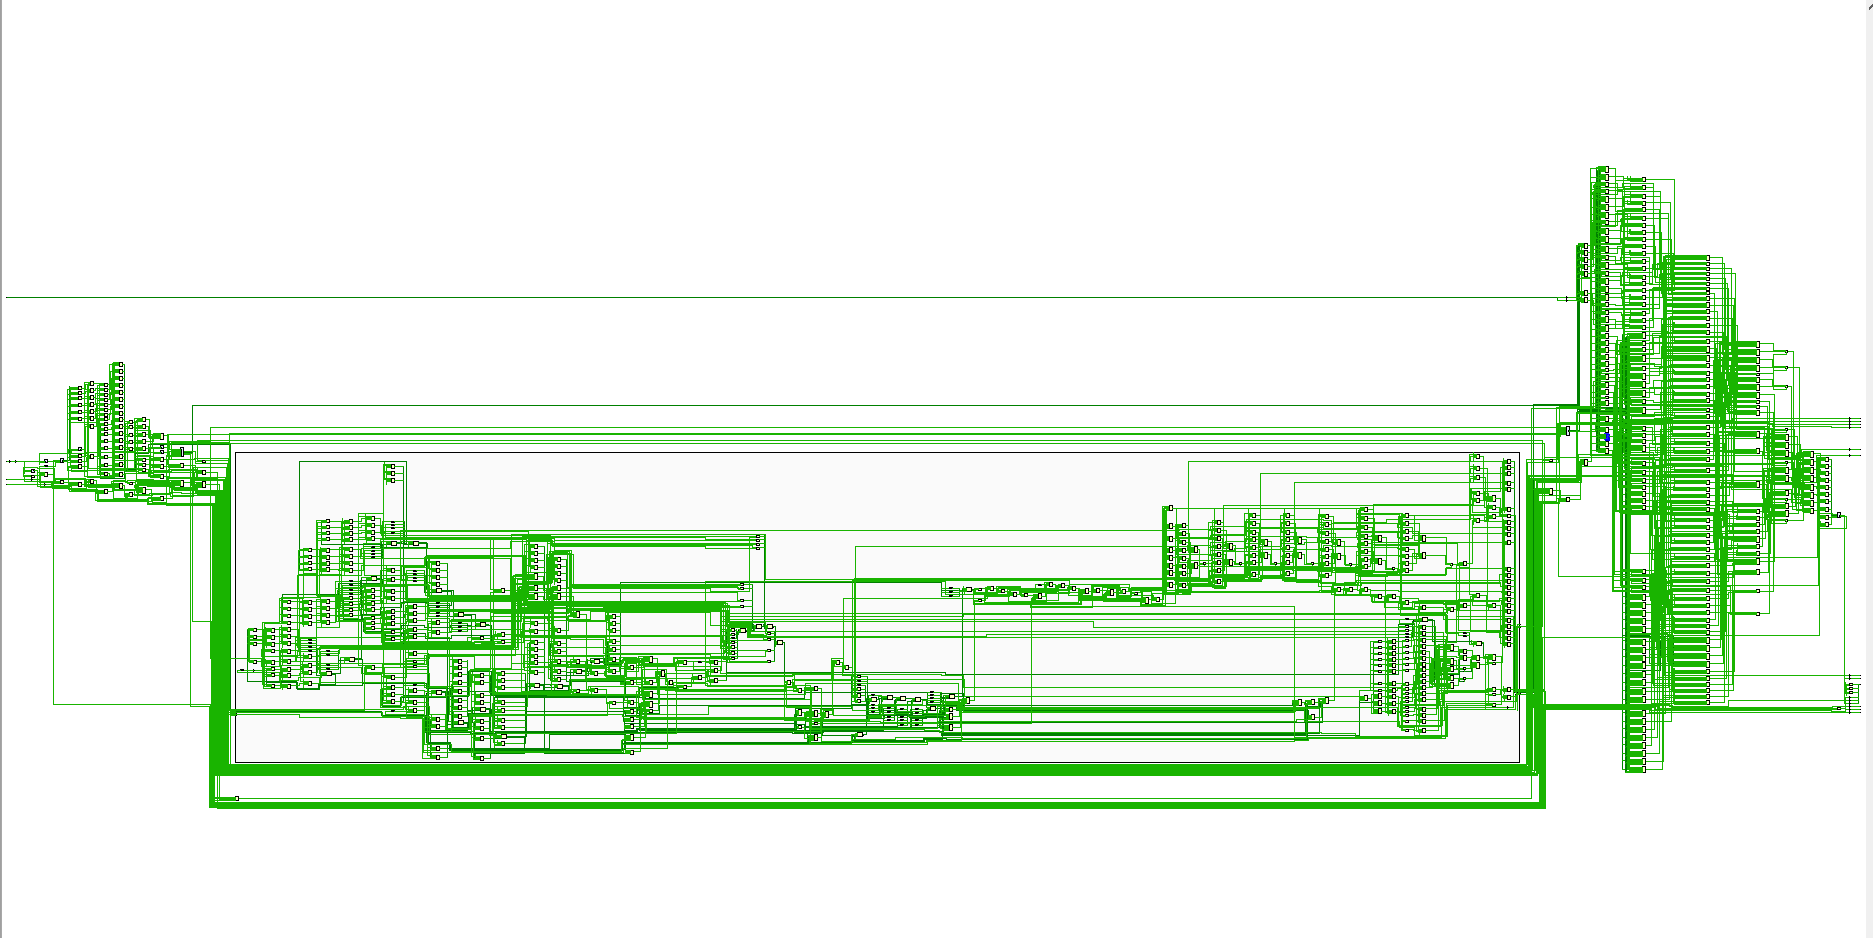
\includegraphics[scale=0.4]{fpga_synth_canexpand}
%\hspace{1em}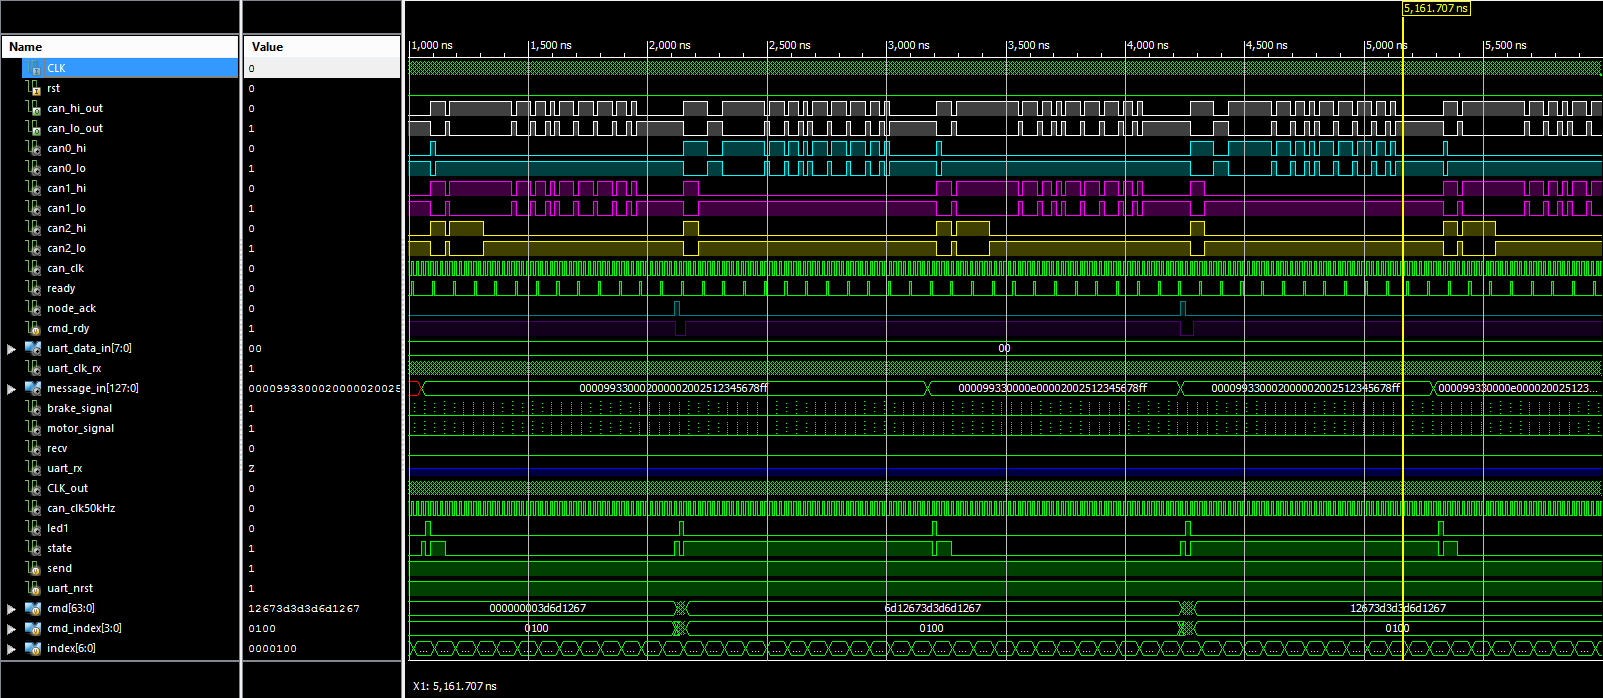
\includegraphics[scale=0.5]{FPGA_Sim1}
\hspace{5em}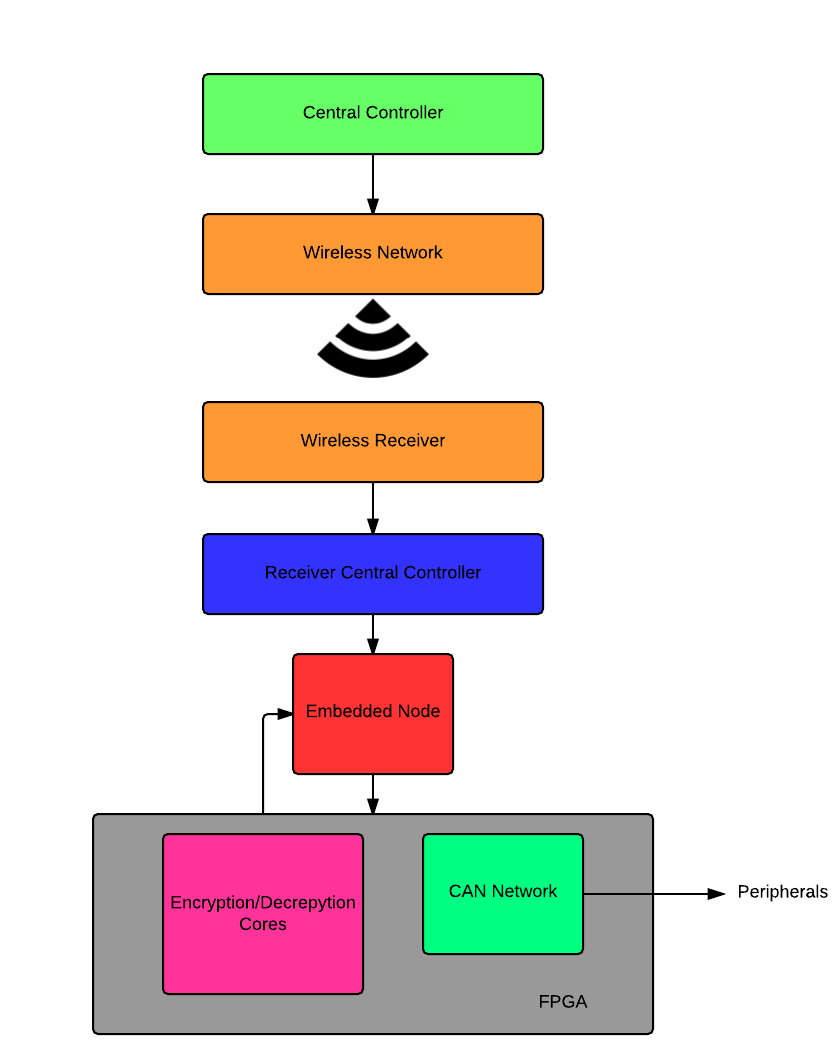
\includegraphics[scale=1.1]{design_flow}
\end{vwcol}

%\centerline{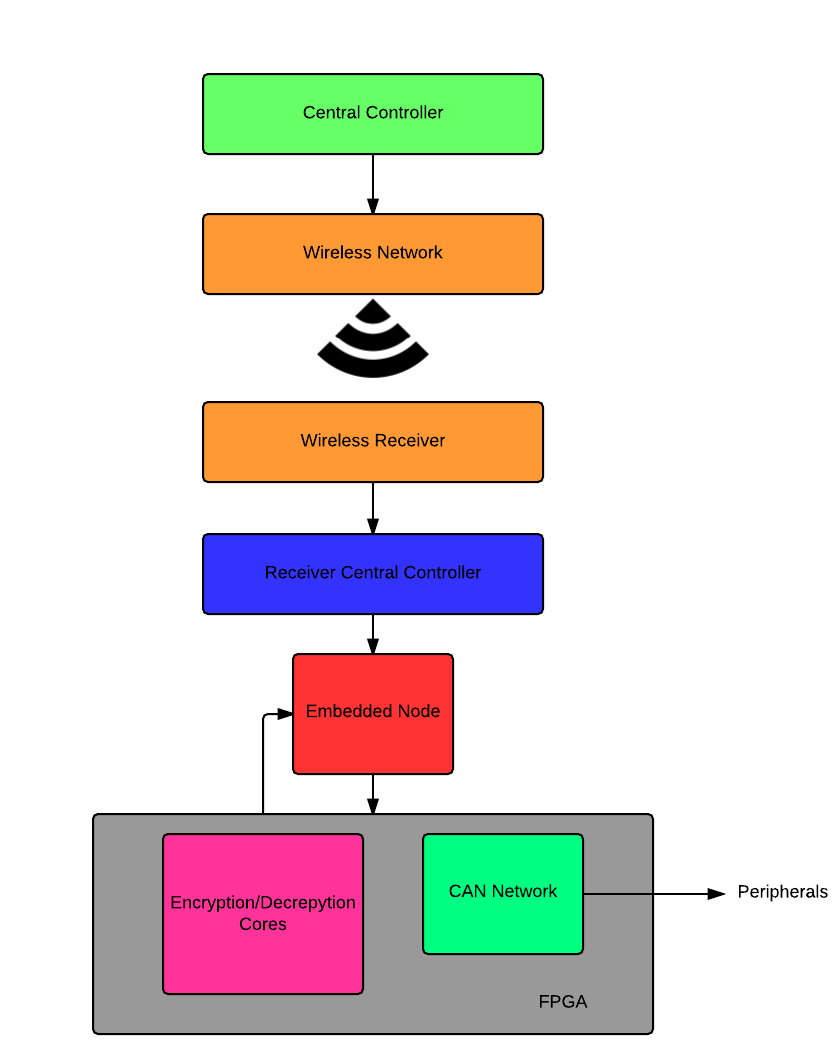
\includegraphics[width=0.6\linewidth]{design_flow}}

\centerline{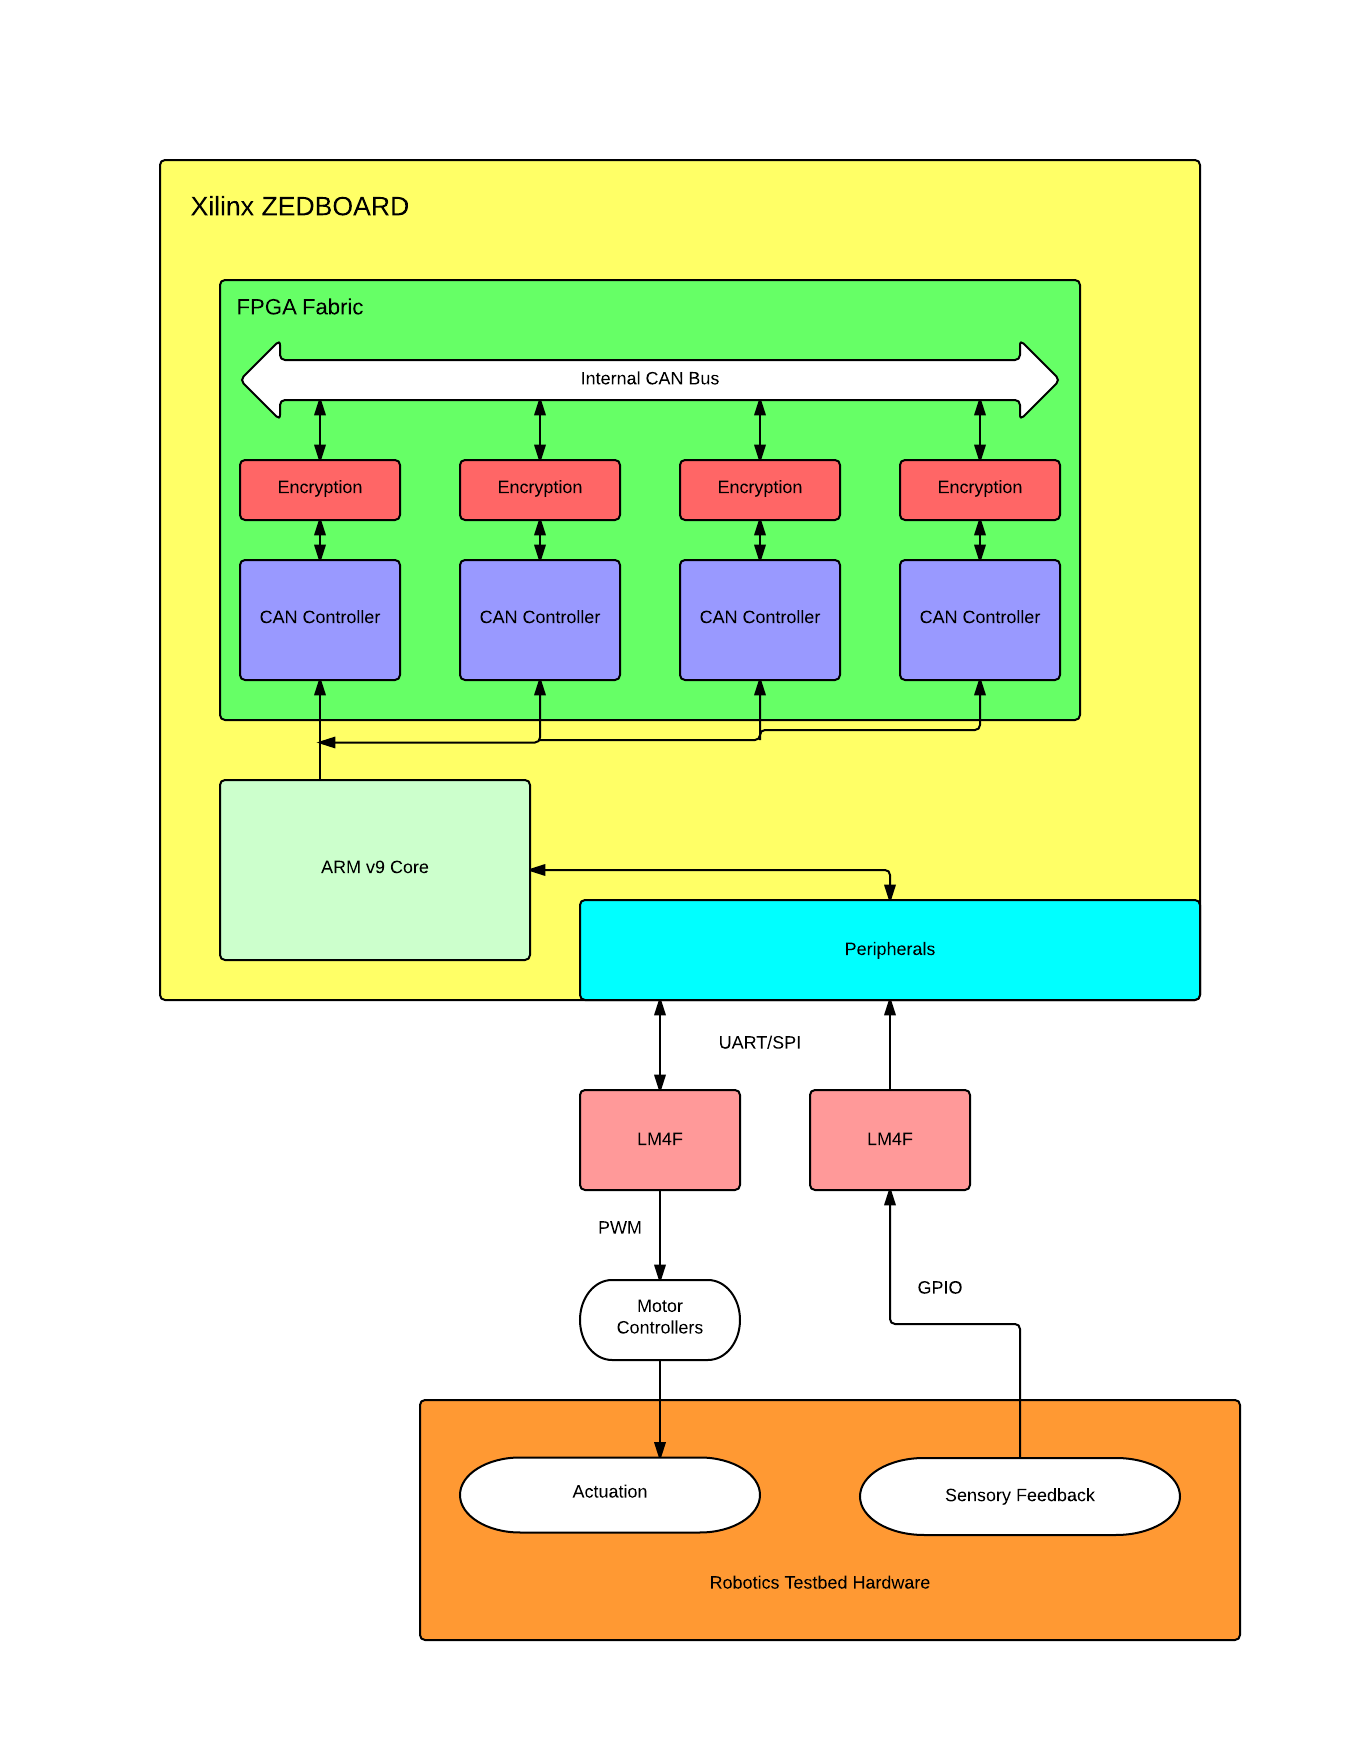
\includegraphics[scale=0.9]{fpga_layout}}
%\bf{Figure 1. } FPGA Layout
\vspace{1em}
\centerline{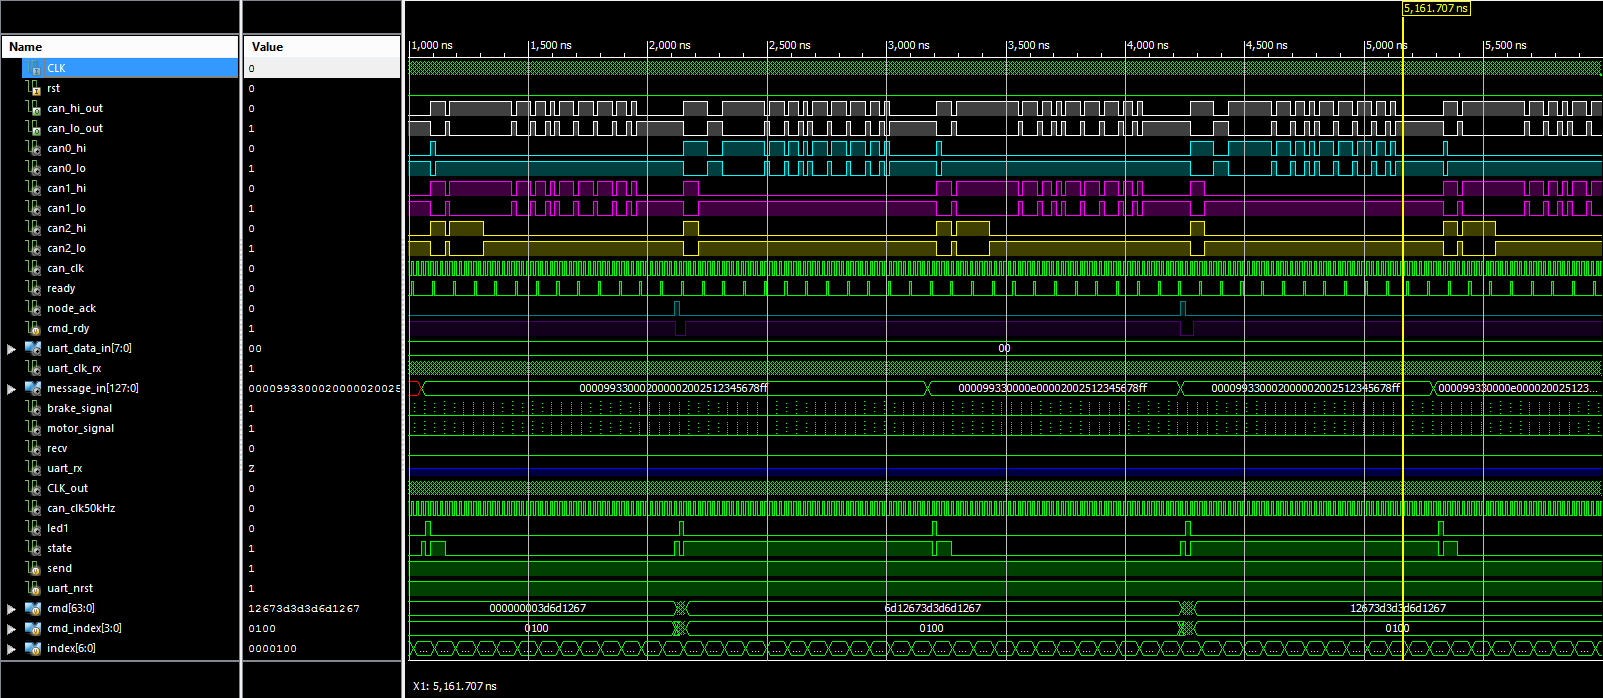
\includegraphics[width=0.9\linewidth]{FPGA_Sim1}}
%\vspace{-1em}

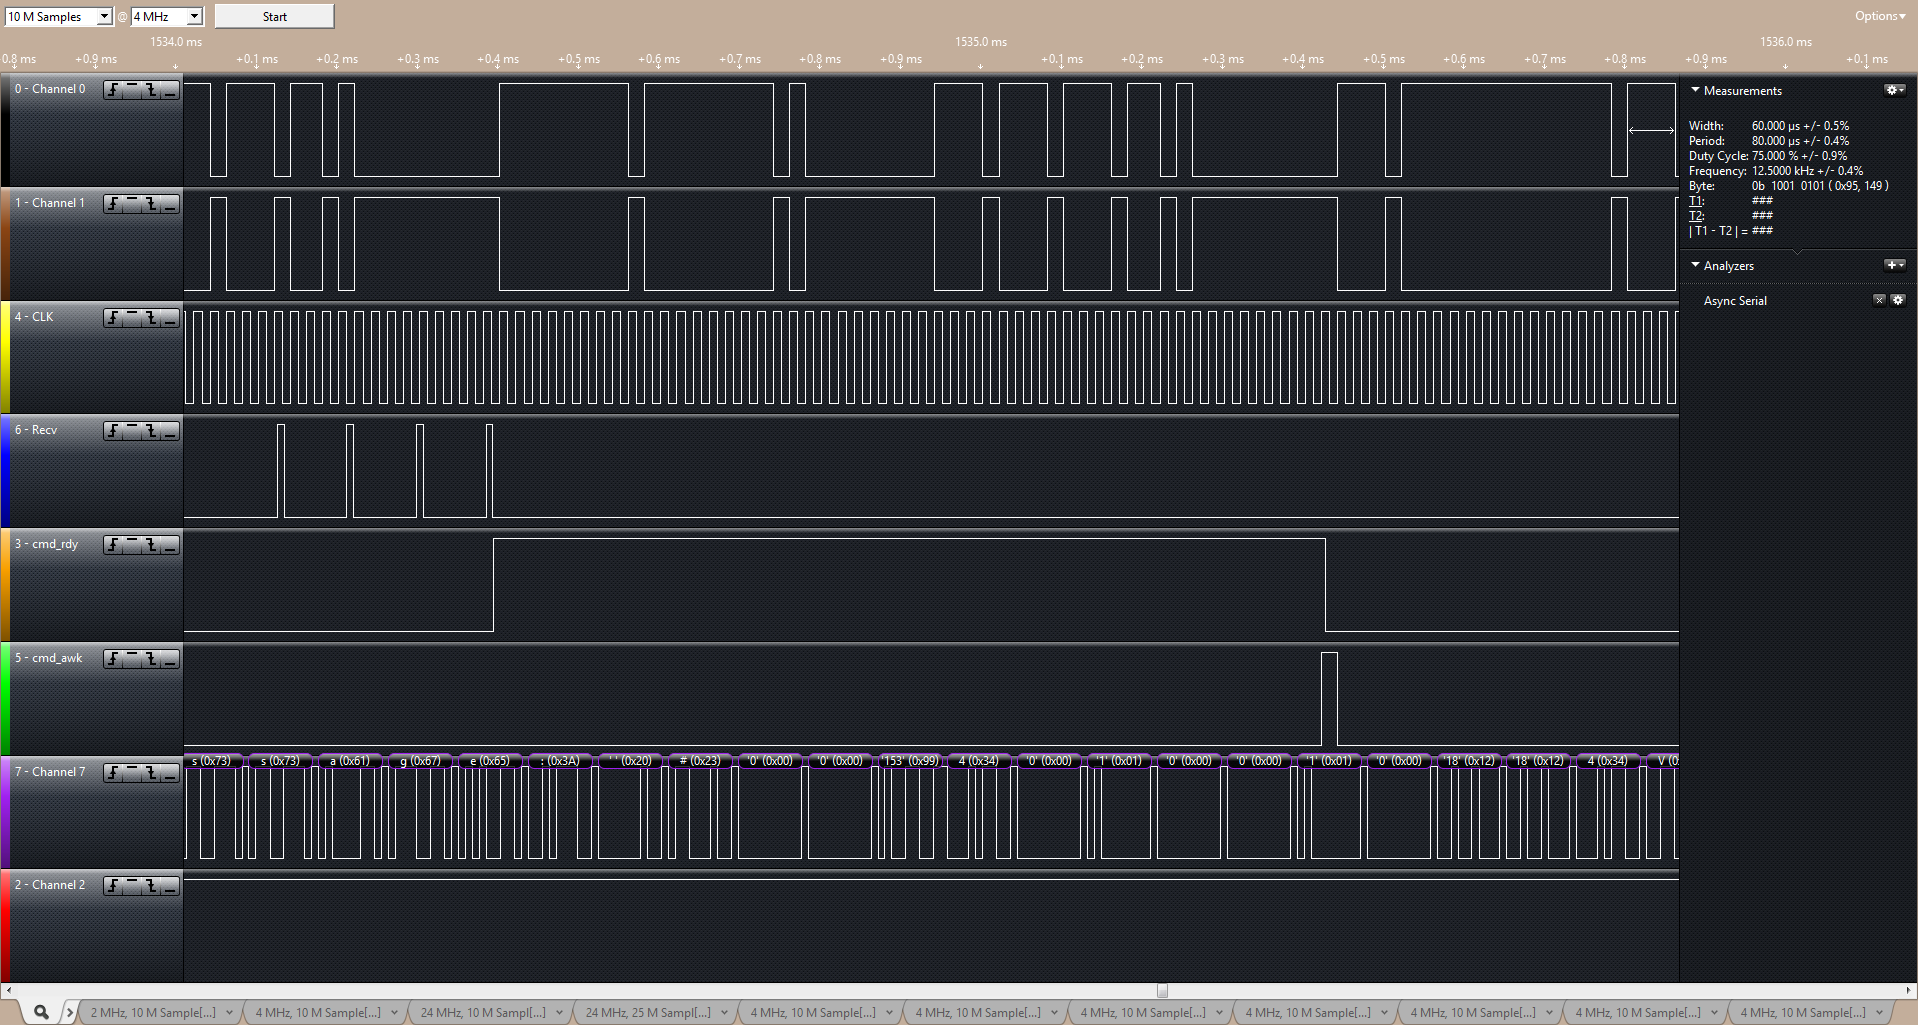
\includegraphics[width=0.9\linewidth]{UART-CAN_PacketTranslation}
\\
%\bf{Figure 2. } Hardware CAN Bus Capture

\centerline{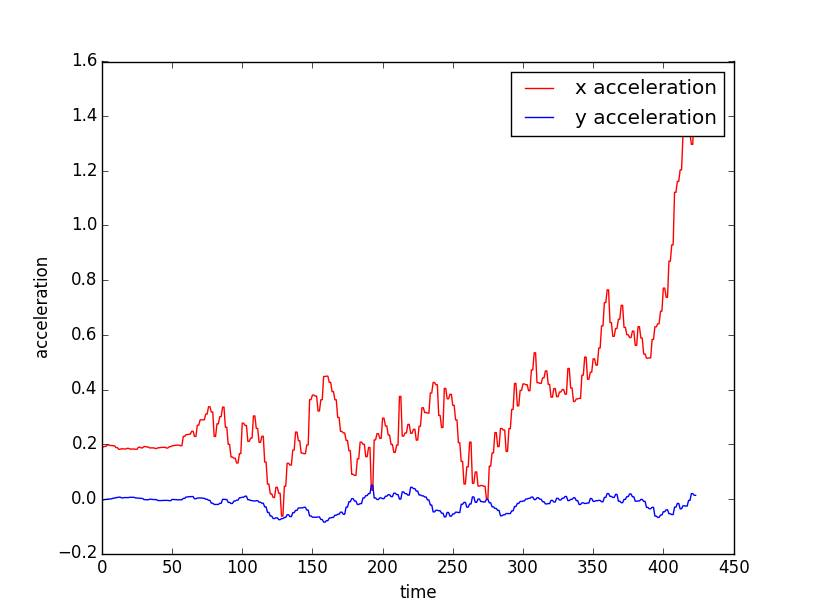
\includegraphics[scale=0.7]{imu_plot2}}


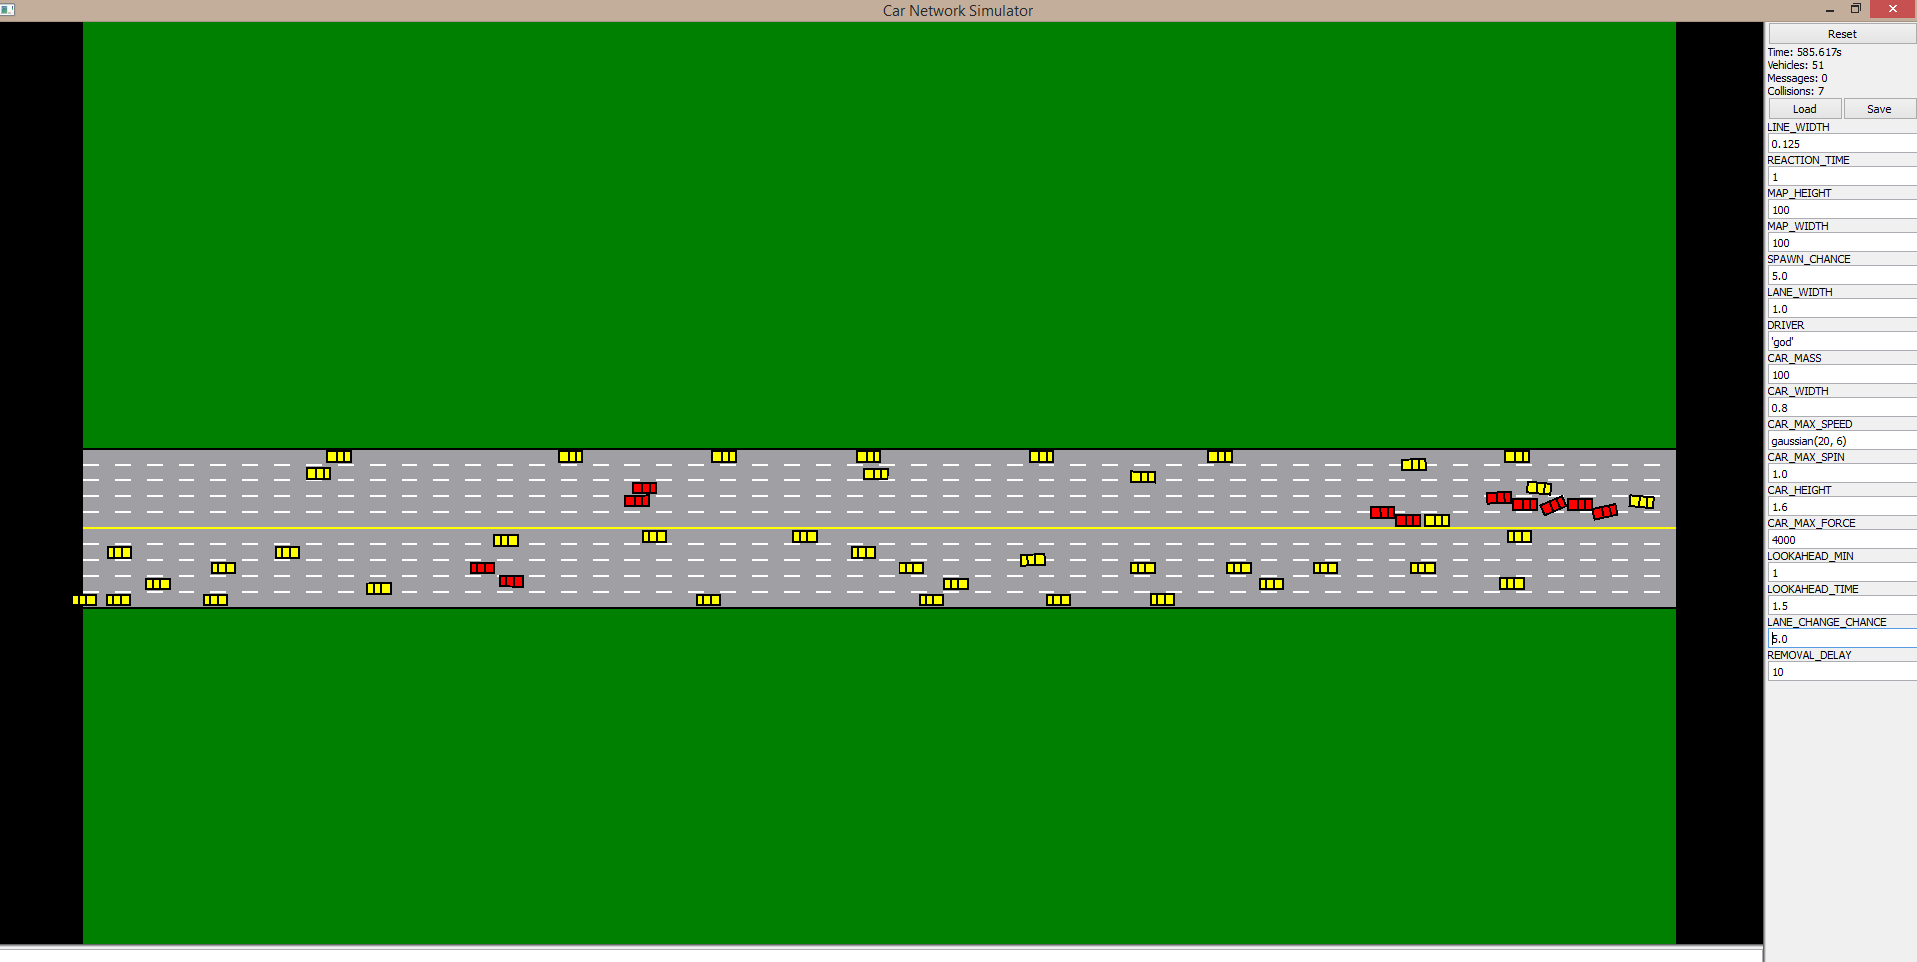
\includegraphics[width=1\linewidth]{car_sim}


%	RESULTS 
%----------------------------------------------------------------------------------------

\section*{Results}
Software encryption was shown to be extremely slow, taking upwards of 8.9 seconds to scramble data using a simple cipher. In addition during wireless transmission, using an ad-hoc (typically used for long term secure channels) took several seconds on average to connect. This would not be a feasible communication method at high speeds. Utilizing high frequency channels similar to DSRC would allow for rapid bursts of data, while using hardware encryption would provide ciphertext at the rate of between 20-100ns for a 128-bit block (using a tiny AES-256 core on a Xilinx Zync FPGA running at 50MHz).
%Latency in the system was measured by sending commands via the transceivers, forwarding the packet via USB-UART to an embedded node which would run a PID loop, forwarding data through a separate UART module to the FPGA. The FPGA would in turn construct a CAN frame around the incoming data after performing an ID-table lookup to confirm a valid message and transmits the data. The correct listening node can then interpret the command and interface with the peripherals on the testbed via a PWM signal. Encryption/Decryption blocks were configured as a feedback loop, taking in plaintext data via a separate dedicated UART line and piping the scrambled data back up through to the central controller.


%----------------------------------------------------------------------------------------
%	CONCLUSIONS
%----------------------------------------------------------------------------------------

\color{SaddleBrown} % SaddleBrown color for the conclusions to make them stand out

\section*{Conclusions}
Vivamus molestie, risus tempor vehicula mattis, libero arcu volutpat purus, sed blandit sem nibh eget turpis. Maecenas rutrum dui blandit lorem vulputate gravida. Praesent venenatis mi vel lorem tempor at varius diam sagittis. Nam eu leo id turpis interdum luctus a sed augue. Nam tellus.


%----------------------------------------------------------------------------------------
%	ACKNOWLEDGEMENTS
%----------------------------------------------------------------------------------------

\section*{Acknowledgements}

Dr. Tiwari, TI, UT Austin, swiggity swaggity swoop

%----------------------------------------------------------------------------------------

\end{multicols}
\end{document}
